
\chapter{Teori}

I detta kapitel beskrivs fyra koncept av central betydelse för projektet. Dessa
koncept är domänspecifika språk, begreppen syntax, syntaxträd och semantik,
litterat programmering samt lärandeteorier.

\section{Domänspecifika språk}

Ett domänspecifikt språk är ett språk som är avgränsat till en specifik domän.
Nyckelorden är språk, specifik och domän. En domän är ett område, till exempel
textformatering eller matlagning. Specifikt syftar det på att det är \textit{just
detta} område som fokus läggs på. Med språk menas ett sätt att uttrycka
saker inom domänen. Svenska och Java är två exempel på språk.
Domänspecifika språk är vanligt förekommande i programmeringssammanhang, HTML är
ett domänspecifikt språk för textformatering, SQL för databashantering och
CSV för tabeller.

Domänspecifika språk används inte bara i programmering utan förekommer även i
andra mer vardagliga sammanhang. Inom domänen matlagning är steka, grilla och
fritera användbara ord, likaså inom domänen ridning är grimma, box och galopp
användbara ord. Är personen bekant med domänen vet den vad som menas med grimma
och det är ett kort och väldefinierat sätt att uttrycka sig. Men detta språk (här
i form av ord och begrepp) blir svårtolkat utanför domänen. Ett recept kan inte
förklaras i termer av grimmor, boxar och galopper.
Precis som domänspecifika språk i vardagen passar
domänspecifika språk inom programmering bäst för sin egen domän. SQL är bra för
att hantera en databas men inte för att skapa ett spel.

Motsatsen till ett domänspecifikt språk är ett generellt språk. I
vardagen är naturliga språk som svenska och engelska generella medan
ryttarbegreppen ovan är domänspecifika. Precis som i vardagen finns
det i datavärlden generella programmeringsspråk, till exempel C++ och
Java. Dessa språk har inte en specifik domän utan kan användas till flera olika, Java kan till exempel användas till både databaser och spel. Nackdelen med
dessa generella språk är just att de är så generella. Eftersom
domänspecifika språk inte behöver vara användbara utanför den
specifika domänen kan de inkludera specifik syntax och ha en inbyggd
funktionalitet som inte hade passat i ett generellt språk.

Ett domänspecifikt språk kan antingen implementeras som ett fristående språk
eller bäddas in i ett redan existerande språk. De domänspecifika språk som
utvecklats inom detta projekt är inbäddade i programmeringsspråket
\textit{Haskell}. Haskell är ett lämpligt val eftersom det är enkelt att skapa
datatyper som bygger upp det domänspecifika språket. Att Haskell är ett
högnivåspråk är också en fördel då programmeraren slipper programmeringstekniska detaljer som
minneshantering och kan istället fokusera på programmets innehåll
och betydelse. Slutligen möjliggör mönstermatchning att de konstruktorer som bygger
upp datatyperna i det domänspecifika språket enkelt kan brytas isär och manipuleras.

För vidare läsning om domänspecifika språk rekommenderas \textit{DSL for the Uninitiated}~\cite{DSLU}.

\section{Syntax, syntaxträd och semantik}\label{sec:syntax}

I samband med domänspecifika språk dyker begreppen \textit{syntax} och
\textit{semantik} upp. Syntax är reglerna för hur enheter i språket, till exempel ord och skiljetecken, sammanslås till komplexa strukturer som meningar och
satser. Semantiken är betydelsen av sådana komplexa strukturer i ett språk.
Inom aritmetik\footnote{Aritmetik är
  den gren inom matematiken som behandlar räkning av tal.} är tal och
operationer syntax medan värdet av uttrycket är semantiken.  Till
exempel har det syntaktiska uttrycket $((3 + 2) * 10)^4$ det semantiska värdet $6.250.000$,
eftersom det är det som det syntaktiska uttrycket \textit{betyder}.
Domänspecifika språk har med syntax att göra eftersom många
domänspecifika språk används för att modellera just syntax.

I domänspecifika språk som modellerar syntax, så kallade \textit{deep
embeddings}, kan syntaxen representeras av trädstrukturer. Dessa
strukturer kallas \textit{syntaxträd}, och har haft stor betydelse i detta projekt.
För att illustrera begreppet visas här ett domänspecifikt språk som består av en
datatyp vars element är
syntaxträd som modellerar aritmetiska uttryck, implementerat i Haskell.
Datatypen för syntaxträden visas i figur~\ref{fig:syntax_exempel}.

\begin{figure}[tph]
  \begin{lstlisting}
data Expr = Expr :+: Expr
          | Expr :*: Expr
          | Const Double
  \end{lstlisting}
  \caption{En datatyp för aritmetiska uttryck i Haskell. Detta är ett exempel på
           ett litet domänspecifikt språk.}\label{fig:syntax_exempel}
\end{figure}

Typen innehåller \textit{datakonstruktorer} för att representera
\textit{löv} (ändpunkter) och \textit{förgreningar}. I detta exempel är
\texttt{:+:} och \texttt{:*:} förgreningar. Med hjälp av dem kan summan respektive produkten av två andra uttryck uttryckas. Löven
% Löfven
representeras av
\texttt{Const}, vilket är en konstant som ej kan byggas vidare på\todo{Const 10 :*: Const 2??}.

Med datakonstruktorerna kan uttryck representerade av syntaxträd konstrueras. Ett exempeluttryck
från den tidigare datatypen visas i figur~\ref{fig:syntax_exempel_varde}, där det aritmetiska uttrycket $7 * (3
+ 10)$ modelleras. Konstruktorn \texttt{:*:} får som sina två argument uttrycken
\texttt{Const 7} och \texttt{Const 3 :+: Const 10}. Det är alltså en produkt av
två deluttryck. Syntaxträd brukar illusteras med träddiagram. Detta
exempeluttryck illustreras i figur \ref{fig:syntax_exempel_bild}.

\begin{figure}[tph]
  \begin{lstlisting}
expr = Const 7 :*: (Const 3 :+: Const 10)
  \end{lstlisting}
  \caption{Ett exempeluttryck ur det tidigare syntaxträdet\todo{Vilket syntaxträd?}. Detta modellerar det
           matematiska uttrycket $7 * (3 + 10)$}\label{fig:syntax_exempel_varde}
\end{figure}

\begin{figure}[tph]
  \centering
  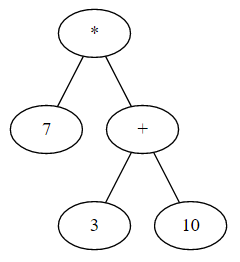
\includegraphics[width=0.4\linewidth]{figure/syntax_exempel_bild.png}
  \caption{Ett exempeluttryck från syntaxträdet\todo{Vilket syntaxträd?} illustrerat i ett
           träddiagram.}\label{fig:syntax_exempel_bild}
\end{figure}

Precis som semantik har en roll i samband med syntax, har semantik även en roll
i samband med syntaxträd. I detta exempel är semantiken det värde som
syntaxträdet har. Detta värde kan beräknas utifrån syntaxträdet genom
en \textit{evaluator}, också kallad \textit{beräkningsfunktion}. För \texttt{Expr}
kan beräkningsfunktionen se ut som i figur \ref{fig:eval_tree}

\begin{figure}[tph]
  \begin{lstlisting}
evaluate :: Expr -> Double
evaluate (e1 :+: e2) = evaluate e1 + evaluate e2
evaluate (e1 :*: e2) = evaluate e1 * evaluate e2
evaluate (Const v)   = v
  \end{lstlisting}
  \caption{En beräkningsfunktion för syntaxträdet.}\label{fig:eval_tree}
\end{figure}

Det finns tre speciella saker att observera i
figur~\ref{fig:eval_tree}. Den första är att eftersom syntaxen innehåller tre olika
slag av element, här motsvarat av de tre datakonstruktorerna, krävs tre fall i
funktionen \texttt{evaluate} som beräknar vardera av dem. Den har
därför ett fall för \texttt{:+:}, ett för \texttt{:*:} och ett för
\texttt{Const}.

Den andra saken att notera i figuren är hur ett fall
beräknas. Hur beräkningen ska se ut fås genom att ta hänsyn till
semantiken hos det syntaktiska uttrycket. Här är \texttt{e1 :+: e2} syntax för
addition av de två uttrycken \texttt{e1} och \texttt{e2}. Därför blir
semantiken, värdet, av \texttt{e1 :+: e2} lika med värdet hos \texttt{e1} och
\texttt{e2} adderade. Ett liknande resonemang ger svaret på hur beräkningen av
de två resterande fallen ska se ut.

Den tredje saken värd att poängtera är beräkningsfunktionens
typsignatur, \texttt{Expr -> Double}. Den gör nämligen att
\texttt{evaluate}, och beräkningsfunktioner i allmänhet, kan tolkas som en översättning
från syntax (här \texttt{Expr}) till semantik (här \texttt{Double}).

\section{Litterat programmering och Literate Haskell}\label{sec:lhs}

\textit{Litterat programmering} (engelska \textit{literate programming}) är ett
alternativt sätt att programmera som introducerades av Donald Knuth~\cite{knuth}.
Istället för att skriva ett program främst för datorer att exekvera, så skrivs
programmet främst för människor att läsa.

Jämfört med traditionella program får dokumentationen en
ökad betydelse. I traditionella program är programkoden den viktiga delen. I
litterata program är däremot dokumentationen minst lika viktig. Den används för
att förklara koden, sätta den i relation till andra delar, med mera.
Detta jämnbördiga förhållande syns konkret genom att titta på hur källkoden är
skriven i ett litterat program. Det kan till exempel se ut som i
figur~\ref{fig:litterate_haskell_exempel} där källkoden och
dokumentationen är sammanvävda på ett jämnbördigt sätt, där den ena inte är
viktigare än den andra.

\begin{figure}[tph]
  \begin{lstlisting}[language={}]
How does all this tie together? First the type is decided, for instance

> type ExampleType = Quantity T.Length Double

then a value of that type is created

> exampleValue :: ExampleType
> exampleValue = Quantity V.length 5.3

Note that the Quantity data type has both value-level and type-level dimensions. As previosuly mentioned, value-level in order to pretty print and type-level to only permit legal operations.
\end{lstlisting}
  \caption{Ett exempel på hur en källfil till litterat programmering kan se ut, tagen direkt från källkoden till läromaterialet.
           I exemplet är koden skriven i Literate Haskell. Rader som börjar med \texttt{>}
           markerar att det är programkod, medan rader utan markerar att det är
           dokumentation.}\label{fig:litterate_haskell_exempel}
\end{figure}
% OBS! Raden med "note that the quantity..." måste vara en lång rad. Annars blir det fel i PDF:en

%Det andra sättet ett litterat program skiljer sig åt är ordningen programkoden
%står i. Traditionell programmering börjar oftast med att definiera små funktioner
%och metoder med snäva användningsområden och använder sedan dessa för att senare
%bygga ihop mer komplexa strukturer. Med litterat programmering börjar man hellre
%med komplexa strukturer först och skriver text som förklarar den generella
%strukturen utan att gå in på detaljerna, för att sedan presentera de små
%delarna var för sig med tillhörande förklarande text.

\textit{Literate Haskell} är litterat programmering för Haskell~\cite{litterate_haskell}.
Att programmera i Literate Haskell går till på samma sätt som vanlig Haskell,
med skillnaden att programkod och text vävs ihop i en och samma fil. Det kan
se ut som i figur~\ref{fig:litterate_haskell_exempel}. Filen, med tillägget
\texttt{.lhs}, går att använda direkt med Haskell-kompilatorn GHC. All text
ignoreras och programkoden behandlas som om den var en vanlig
Haskell-fil. Filen kan också kompileras till en läsbar typsatt rapport eller hemsida.
Det som används i detta
projekt är \textit{Pandoc}~\cite{pandoc}. Med Pandoc kan texten märkas
upp med både \textit{Markdown} (används i projektet) och \LaTeX. Det går
att exportera till bland annat HTML (som i läromaterialet) och PDF (som i den här rapporten).


\section{Lärandeteorier}\label{sec:arcs}

Motivation är en persons vilja att göra något och i undervisningssammanhang vill
läraren eller författaren att studenten ska lära sig materialet, studenten behöver alltså bli
motiverad till att lära sig. Motivation kan ha flera källor, till exempel
att studenten tycker materialet är intressant eller att det finns belöningar i
form av tillfredsställelsen från ett högt betyg.

\textit{Motiverande design} innebär att systematiskt utforma undervisningen på
ett sådant sätt att studenten blir motiverad till att lära sig. Det handlar om
att använda olika tekniker för att väcka och behålla motivation. För detta finns
det ett flertal olika modeller men i detta projekt används enbart den så
kallade \textit{ARCS-modellen}~\cite{arcs_book}.

\textit{ARCS} är en förkortning av ``Attention, Relevance, Confidence and
Satisfaction'', på svenska ``uppmärksamhet, relevans, självförtroende och
tillfredsställelse''. Precis som namnet antyder innehåller modellen fyra delar
som vardera behandlar en aspekt av motivation.
\begin{itemize}
  \item \textit{Attention} handlar om att fånga uppmärksamhet och väcka
    nyfikenhet.
  \item \textit{Relevance} handlar om att tillgodose studentens behov så
    att materialet upplevs som relevant.
  \item \textit{Confidence} handlar om att övertyga studenten att hen kan lyckas
    lära sig materialet.
  \item \textit{Satisfaction} handlar om att ge studenten
    tillfredsställelse efter att ha lärt sig något så att hen vill fortsätta
    lära sig.
\end{itemize}
Det finns olika strategier för hur de olika delarna genomförs i praktiken,
här följer en översikt för \textit{Attention}\footnote{Eftersom projektet har
ett begränsat fokus på de pedagogiska aspekterna, se
avsnitt~\ref{sec:avgransningar}, har enbart \textit{Attention} tagits hänsyn
till. Av detta skäl är enbart denna del beskriven här.}.

För att fånga studentens uppmärksamhet och intresse finns tre allmänna
strategier. Den första är varseblivning, att något plötsligt händer som studenten
blir medveten om. Det kan till exempel åstadkommas genom överraskande
information, en förändring i ljuset i en föreläsning eller att humor vävs in.
Den andra är att väcka nyfikenhet. Ett par sätt för det är att involvera mystik
i miljön och att ställa frågor. Det tredje sättet är variation. Då handlar det
om olika struktur och ordning på undervisningen, till exempel att inte alltid
utforma en lektion som föreläsning, demonstration och sedan övning, utan variera
det med andra inslag, exempelvis ett filmklipp.
\todo{Röd tråd}
Enligt det sociokulturella perspektivet som Vygotskij utvecklade~\cite{LSB_und}
lär sig elever av varandra. Eleverna befinner sig vid sin närmsta
utvecklingszon\footnote{Den zon där målet för lärandet ligger på en nivå som är
för hög för en elev att klara på egen hand, men som eleven klarar om den får
vägledning och stöd.}, där eleverna kan hjälpa varandra att förstå innebörden av
definitioner och uttryck genom att sätta ord på det de vill kommunicera. Denna
typ av kommunikation kan hjälpa elever sätta fingret på vad de
inte förstår. Med denna bakgrund kan parprogrammering vara
fördelaktigt. Dels för att eleverna kan lära sig av varandra, dels för att de genom att
kommunicera
%sin förståelse
internaliserar ämnet och bygger en djupare
förståelse. Parprogrammering kan även lämpa sig för att begränsa
flyktförsök, där elever medvetet eller mindre medvetet börjar ägna sig åt något annat.

%Jean Piaget - Kognitivismen (lära sig A, B, A + B -> C, alternativt att eleven utmanas med något den trodde var sant, och tvingas omformulera en lösning som stödjer den presenterade situationen). s157

Två andra aspekter på lärande är interaktion och snabba
belöningar. Eftersom internetplattformars interaktion med eleven är
begränsad i jämförelse med då eleven är i skolan och har tillgång till
lärare, så brukar internetbaserade läroplattformar förlita sig på
behavioristiska element (former av respons) i form av rätt eller fel
svar~\cite{LSB_und}. Evolutionärt sett har snabba belöningar varit
fördelaktigt framför långsiktiga som kräver långsiktigt engagemang
(exempelvis öva inför en tenta) vilket beskrivs i boken \textit{Dansa
på deadline: Uppskjutandets psykologi}~\cite{DPD}.\todo{Oavslutat stycke}
